\section{Positive partitions and a wider asymptotic window}\label{sec:extension}

The recurrence admits a positive coefficient representation. It explains the hyperbolic functions by counting pairs and triples, and extends their relative accuracy well beyond the critical cubic range. At the square-root scale, a further correction becomes visible.

For $k\ge2$, put $m=\lfloor k/2\rfloor$, $K=2m$ and
\begin{equation}\label{eq:hyperdef}
\lambda=\frac23\sqrt{K^3/N},\qquad
H_k=\begin{cases}\cosh\lambda,&k\text{ even},\\
\shc\lambda,&k\text{ odd}.
\end{cases}
\end{equation}
For odd $k$, the definition intentionally uses $K=k-1$.



\begin{theorem}[Relative hyperbolic approximation]\label{thm:window}
For integers $2\le k\le N/4$,
\begin{equation}\label{eq:envelope}
\left(1-\frac{4k^2}{3N}\right)H_k
\le R_k\le e^{4k^2/N}H_k.
\end{equation}
If $4k^2\le N$, then
\begin{equation}\label{eq:logerror}
-\frac{2k^2}N\le\log\frac{R_k}{H_k}\le\frac{4k^2}N.
\end{equation}
Consequently $R_k/H_k\to1$ whenever $k=o(\sqrt N)$, even if $k^3/N\to\infty$.
\end{theorem}

\begin{theorem}[The square-root correction]\label{thm:sqrt}
If $k^2/N\to d\in(0,\infty)$, then
\begin{equation}\label{eq:sqrtlimit}
\frac{R_k}{H_k}\longrightarrow e^{d/4}.
\end{equation}
For every fixed $C>0$,
\begin{equation}\label{eq:uniformsqrt}
\sup_{2\le k\le C\sqrt N}
\left|\frac{R_k}{e^{k^2/(4N)}H_k}-1\right|\longrightarrow0,
\end{equation}
where the supremum is over integers and $N\to\infty$.
\end{theorem}

Thus the uncorrected hyperbolic approximation loses relative accuracy at every positive square-root scale. The corrected expression is uniformly accurate on bounded multiples of that scale. Sections~\ref{sec:asymptotics} and~\ref{sec:rates} extend its range and determine its sharp first error.

\subsection{Clearing the denominators}

Set $Q_k=(N)_kN^ka_k$, with $Q_0=1$ and $Q_1=0$. Equation~\eqref{eq:momentrec} becomes
\begin{equation}\label{eq:qrec}
Q_k=2(k-1)Q_{k-1}+(k-1)(N-k+2)Q_{k-2}.
\end{equation}
Extend this polynomial recurrence formally to all orders. This algebraic extension does not define permutation moments for $k>N$. The exponential generating function $F(z)=\sum_{k\ge0}Q_kz^k/k!$ satisfies
\[
(1-z)^2F'(z)=NzF(z),\qquad F(0)=1.
\]
Consequently,
\begin{equation}\label{eq:egf}
F(z)=\exp\left(N\left[\frac z{1-z}+\log(1-z)\right]\right)
=\exp\left(N\sum_{j\ge2}\frac{j-1}{j}z^j\right).
\end{equation}
This is a classical Laguerre generating function: $Q_k=k!L_k^{(-N-1)}(-N)$ \cite[equations 18.5.12 and 18.12.13]{DLMF}. It is also a reformulation of the special-function identification in \cite[Remark 3.5]{CN}. We derive it here to use its positive coefficients, not as a new special-function identity.

Extracting coefficients gives
\begin{equation}\label{eq:partitions}
Q_k=k!\sum_{\substack{c_2,c_3,\ldots\ge0\\\sum_{j\ge2}jc_j=k}}
\prod_{j\ge2}\frac{(N(j-1)/j)^{c_j}}{c_j!}.
\end{equation}
Equivalently, this is a weighted count of labeled set partitions without singleton blocks. A block of size $j$ has weight $N(j-1)(j-1)!$. Pairs have weight $N$, and triples have weight $4N$.

Define the polynomial leading terms
\[
\mathcal L_{2m}=(2m-1)!!N^m,\qquad
\mathcal L_{2m+1}=\frac{4m}{3}(2m+1)!!N^m.
\]
They count all-pair partitions and one-triple partitions, respectively. Indeed, the latter coefficient is
\[
\binom{2m+1}{3}4(2m-3)!!=\frac{4m}{3}(2m+1)!!.
\]
With $D_k=N^k/(N)_k$, the normalization is exactly
\begin{equation}\label{eq:qnormalize}
R_k=D_k\frac{Q_k}{\mathcal L_k}.
\end{equation}

\subsection{The number of available pairs}

For blocks of size at least three put
\[
S=\sum_{j\ge3}jc_j,\qquad x=\sqrt{K/N},\qquad
\lambda_j=N\frac{j-1}{j}x^j.
\]
In particular, $\lambda_3=\lambda$. Cancelling the pair factorial in \eqref{eq:partitions} against the one in $\mathcal L_k$, the normalized contribution of these nonpair counts is
\begin{equation}\label{eq:availabilityeven}
\frac{(m)_{S/2}}{m^{S/2}}
\prod_{j\ge3}\frac{\lambda_j^{c_j}}{c_j!}
\quad\text{if }k=2m\text{ and }S\text{ is even},
\end{equation}
and
\begin{equation}\label{eq:availabilityodd}
\frac{(m-1)_{(S-3)/2}}{m^{(S-3)/2}}
\frac1\lambda\prod_{j\ge3}\frac{\lambda_j^{c_j}}{c_j!}
\quad\text{if }k=2m+1\text{ and }S\text{ is odd}.
\end{equation}
An odd $S$ here is at least three. A falling factorial with too many factors is assigned zero. The availability factors lie in $[0,1]$ and enforce the requirement that enough pairs remain.

\subsection{Proof of the finite relative bounds}

Assume $k\le N/4$, so $x\le1/2$. Put
\[
A_* =\sum_{\substack{j\ge4\\j\text{ even}}}\lambda_j,
\qquad B_* =\sum_{\substack{j\ge3\\j\text{ odd}}}\lambda_j.
\]
Remove the availability factors and project the exponential series onto the required parity. This gives
\[
\frac{Q_{2m}}{\mathcal L_{2m}}\le e^{A_*}\cosh B_*,\qquad
\frac{Q_{2m+1}}{\mathcal L_{2m+1}}\le e^{A_*}\frac{\sinh B_*}{\lambda}.
\]
The extra block weights satisfy
\begin{align*}
A_*+B_*-\lambda&\le\frac{Nx^4}{1-x}\le\frac{2K^2}N,\\
\frac{B_*}{\lambda}&\le1+\frac{3x^2}{2(1-x^2)}
\le1+\frac{2K}N\le e^{K^2/N}.
\end{align*}
The logarithmic derivatives of $\cosh t$ and $\shc t$ lie in $[0,1]$ for $t>0$. For the latter this follows from $0\le\coth t-1/t\le1$. Thus
\[
Q_k/\mathcal L_k\le e^{3K^2/N}H_k.
\]
Also
\[
\log D_k\le\frac{k(k-1)}{2(N-k+1)}\le k^2/N.
\]
Equation~\eqref{eq:qnormalize} proves the upper bound in \eqref{eq:envelope}.

For the lower bound, retain only pairs and triples. At even order, with $J$ triples,
\[
\frac{Q_{2m}}{\mathcal L_{2m}}
\ge\sum_{\ell\ge0}\frac{\lambda^{2\ell}}{(2\ell)!}
\frac{(m)_{3\ell}}{m^{3\ell}}.
\]
For any integer $s\ge0$,
\[
\frac{(m)_s}{m^s}\ge1-\frac{s(s-1)}{2m}.
\]
This follows from the product bound $\prod_i(1-u_i)\ge1-\sum_i u_i$ for $0\le u_i\le1$. If $s>m$, the left side is zero and the right side is nonpositive.

Normalize $\lambda^J/J!$ on even $J$ by $\cosh\lambda$. Then
\[
\E J=\lambda\tanh\lambda,\qquad
\E J^2=\lambda^2+\lambda\tanh\lambda.
\]
With $s=3J/2$, the relative loss is at most
\[
\frac{9\lambda^2+3\lambda\tanh\lambda}{8m}
\le\frac{3\lambda^2}{2m}=\frac{4K^2}{3N}.
\]
For odd order the analogous series is
\[
\frac{Q_{2m+1}}{\mathcal L_{2m+1}}
\ge\sum_{\ell\ge0}\frac{\lambda^{2\ell}}{(2\ell+1)!}
\frac{(m-1)_{3\ell}}{m^{3\ell}}.
\]
Now $(m-1)_s/m^s\ge1-s(s+1)/(2m)$. Normalize $\lambda^J/J!$ on odd $J$ by $\sinh\lambda$ and use $s=3(J-1)/2$. The relative loss is at most
\[
\frac{9\lambda^2-3\lambda\coth\lambda+3}{8m}
\le\frac{9\lambda^2}{8m}=\frac{K^2}N,
\]
because $\lambda\coth\lambda\ge1$. Multiplying by $D_k\ge1$ proves the lower half of \eqref{eq:envelope}. If its factor is negative, positivity suffices. Finally, $\log(1-4u/3)\ge-2u$ for $0\le u\le1/4$, proving \eqref{eq:logerror} and Theorem~\ref{thm:window}.

\subsection{Proof of the square-root correction}

Suppose $k^2/N\to d\in(0,\infty)$. Let $C_j$, $j\ge3$, be independent Poisson variables with means $\lambda_j$, and put
\[
\Lambda=\sum_{j\ge3}\lambda_j,\qquad S=\sum_{j\ge3}jC_j.
\]
For all sufficiently large $N$, $x<1$, so the total mean is finite and only finitely many $C_j$ are nonzero almost surely. Define
\[
w_{\rm e}(s)=(m)_s/m^s\quad(0\le s\le m),\qquad
w_{\rm o}(s)=(m-1)_s/m^s\quad(0\le s\le m-1),
\]
with value zero outside the respective integer ranges. The exact sums \eqref{eq:availabilityeven} and \eqref{eq:availabilityodd} become
\begin{align}
\frac{Q_{2m}}{\mathcal L_{2m}}
&=e^\Lambda\E\bigl[\1_{\{S\text{ even}\}}w_{\rm e}(S/2)\bigr],\label{eq:poissoneven}\\
\frac{Q_{2m+1}}{\mathcal L_{2m+1}}
&=\frac{e^\Lambda}{\lambda}\E\bigl[\1_{\{S\text{ odd}\}}w_{\rm o}((S-3)/2)\bigr].\label{eq:poissonodd}
\end{align}
Each availability function is evaluated only on its displayed parity event.

First control all block sizes:
\[
\lambda\to\infty,\qquad
\lambda_4=\frac{3K^2}{4N}\to\frac{3d}4,\qquad
\sum_{j\ge5}\lambda_j\le\frac{Nx^5}{1-x}\to0.
\]
Therefore $C_3/\lambda\to1$ in probability, $C_4=O_{\PP}(1)$, and the probability of any larger block tends to zero. Also $\Lambda-\lambda\to3d/4$.

On the event of no larger block, the argument $s$ of either availability function is $3C_3/2+2C_4+O(1)$. Since $\lambda^2/m\to8d/9$, we obtain, on the relevant parity event,
\[
\frac{s^2}{2m}\to d,\qquad \frac sm\to0,\qquad \frac{s^3}{m^2}\to0
\]
in probability. For $s/m\le1/2$, expansion of the logarithm gives
\[
\log w_{\rm e}(s)=-\frac{s(s-1)}{2m}+O(s^3/m^2),\qquad
\log w_{\rm o}(s)=-\frac{s(s+1)}{2m}+O(s^3/m^2).
\]
For example, these follow by summing
$0\le-\log(1-u)-u\le u^2/(2(1-u))$.
Thus each availability factor approaches $e^{-d}$ on its relevant parity event. All factors lie in $[0,1]$, so the corresponding error multiplied by the parity indicator tends to zero in mean.

The Poisson parity identity gives
\[
\PP(S\text{ even})=\frac{1+e^{-2B_*}}2,\qquad
\PP(S\text{ odd})=\frac{1-e^{-2B_*}}2.
\]
Because $B_*\ge\lambda\to\infty$, both probabilities tend to $1/2$. Hence both expectations in \eqref{eq:poissoneven} and \eqref{eq:poissonodd} tend to $e^{-d}/2$. No independence between parity and availability is required.

Since $\cosh\lambda\sim e^\lambda/2$ and $\sinh\lambda\sim e^\lambda/2$,
\[
\frac{Q_k/\mathcal L_k}{H_k}\longrightarrow e^{3d/4-d}=e^{-d/4}.
\]
Finally,
\[
\log D_k=\frac{k(k-1)}{2N}+O(k^3/N^2)\longrightarrow d/2.
\]
Restoring $D_k$ in \eqref{eq:qnormalize} proves \eqref{eq:sqrtlimit}. The three contributions are $3d/4$ from four-blocks, $-d$ from pair depletion and $d/2$ from the permutation probability.

To prove \eqref{eq:uniformsqrt}, suppose its supremum failed to tend to zero. Select a sequence of offending orders and pass to a subsequence on which $k^2/N\to d\in[0,C^2]$. If $d=0$, Theorem~\ref{thm:window} gives convergence to one. If $d>0$, \eqref{eq:sqrtlimit} gives it. Both contradict the selection.

\subsection{A worked partition count}

The first polynomials include
\[
Q_2=N,\quad Q_3=4N,\quad Q_4=3N^2+18N,\quad
Q_6=15N^3+430N^2+600N.
\]
For $Q_6$, the four contributions are
\begin{center}
\begin{tabular}{lr}
\toprule
Block sizes & Contribution\\
\midrule
$2+2+2$ & $15N^3$\\
$3+3$ & $160N^2$\\
$2+4$ & $270N^2$\\
$6$ & $600N$\\
\bottomrule
\end{tabular}
\end{center}
At the cubic scale, triples have bounded effective weight, while four-blocks and pair depletion disappear. Summing an even or odd number of triples gives the two hyperbolic functions. At the square-root scale, the four-block weight and pair depletion survive, producing the correction in Theorem~\ref{thm:sqrt}.

In the intermediate regime $N^{1/3}\ll k\ll\sqrt N$, Theorem~\ref{thm:window} also yields
\[
R_k\sim\tfrac12e^\lambda\quad(k\text{ even}),\qquad
R_k\sim\frac{e^\lambda}{2\lambda}\quad(k\text{ odd}).
\]
At $k\sim\sqrt N$, the ratio to the uncorrected hyperbolic term tends instead to $e^{1/4}\approx1.2840$.

\begin{figure}[htbp]
\centering
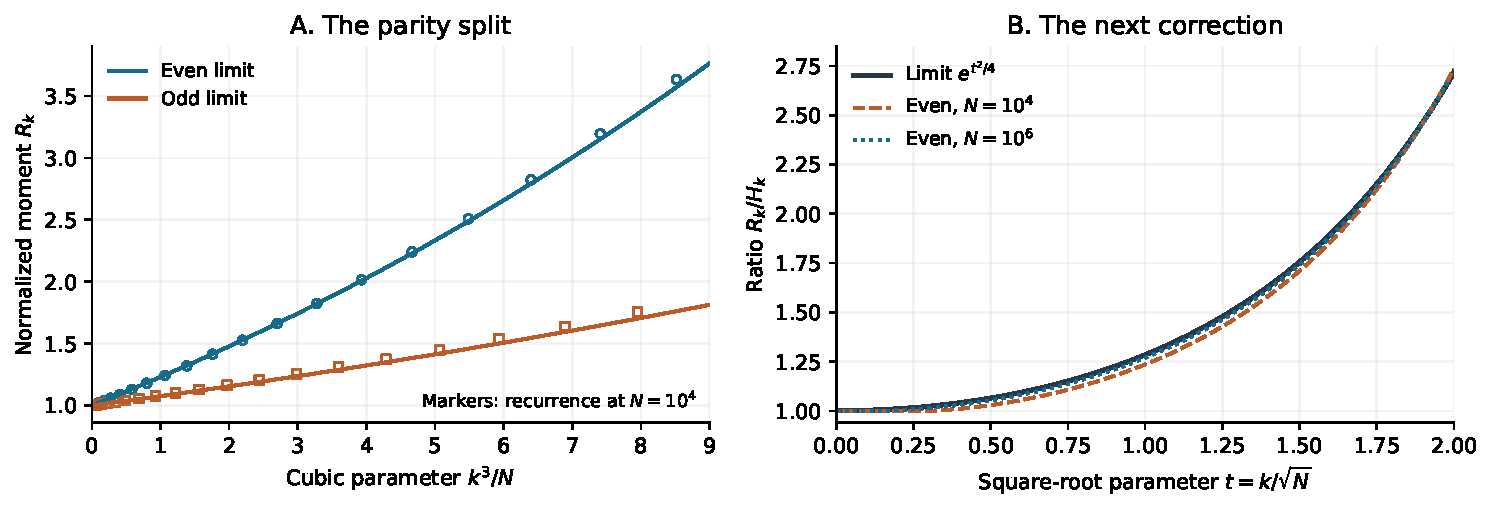
\includegraphics[width=\textwidth]{../figures/moment-regimes.pdf}
\caption{The two transitions. Left: the parity-dependent critical limits and recurrence evaluations at $N=10^4$. Right: the ratio to the hyperbolic approximation at even orders, compared with its square-root correction. Curves illustrate the proved statements and are not premises of the proofs.}
\label{fig:regimes}
\end{figure}
